% Author: Astra
% License: CC0
% From the repository root:
% pdflatex -output-directory build doc/figures/HalfPlaneIntersection.tex
% cp build/HalfPlaneIntersection.pdf content/geometry/HalfPlaneIntersection.pdf
\documentclass[tikz,border=2pt]{standalone}
\usetikzlibrary{arrows.meta}
\begin{document}
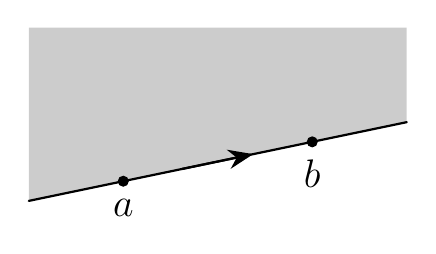
\begin{tikzpicture}[line cap=round, line join=round, >=Stealth]
  % Flat gray marks the included side, cropped to the illustration.
  \fill[black!20] (-2.4,-0.5) -- (2.4,0.5) -- (2.4,1.7) -- (-2.4,1.7) -- cycle;
  % a and b are points on the infinite boundary, not its endpoints.
  \draw[line width=0.8pt] (-2.4,-0.5) -- (2.4,0.5);
  \draw[-{Stealth[length=9pt,width=7pt]},line width=0.8pt]
    (-0.45,-0.09375) -- (0.45,0.09375);
  \fill (-1.2,-0.25) circle (2pt) node[below=3pt,font=\Large] {$a$};
  \fill (1.2,0.25) circle (2pt) node[below=3pt,font=\Large] {$b$};
\end{tikzpicture}
\end{document}
